\chapter{Fundamentals}
\label{cha:fundamentals}

This section describes the fundamental building blocks of the algorithm described in this thesis. It provides a quick overview and explains how the two different simulation techniques work in isolation. It does not describe in any way how the two different simulations might interact but instead it describes them in total isolation.

\section{Rigid Body Simulations}
\label{sec:rigid_body_simulations}

The following section gives a short introduction to rigid bodies simulations largely based on work by Baraff in \cite{Baraff:1997uh} and \cite{Baraff:1997wq}. These notes also form the basis for the rigid body parts implemented as part of the demo application provided by this thesis.

Rigid bodies simulations are very similar to simple particle simulations. Simple particles are modeled as infinitesimal point masses, rigid bodies are additionally defined by their dimension. This extension in space remains constant throughout the whole simulation. A rigid body can therefore be thought of as a set of many particles. When a force acts on any of these point masses all the other connected masses in the rigid body are affected as well. Each point mass has a fixed mass $m_i$ and is located at a fixed position $r_i$ inside the system. The total mass of the rigid body is then simply the sum of all the point masses combined:

\begin{equation}
M = \sum\limits_{i=1}^N m_i
\end{equation}

The position of the particles is defined relative to a local body coordinate system. The origin of the coordinate system is the center of mass the rigid body's mass. The center of mass is calculated as:

\begin{equation}
c = \frac{\sum m_i r_i}{M}
\end{equation}

In order to describe a rigid body simulation two variables are of central importance. Firstly the position \(x(t)\) of the rigid body in space. The second is the orientation \(q(t)\)in space. Both these variables are defined in relation to the world coordinate system. There are two different approaches to model the orientation of the rigid body, either a rotation matrix $R(t)$ or a unit quaternion $q(t)$. In practice almost all cases, unit quaternions are used for a number of reasons. One important aspect is the fact that quaternions do not suffer from gimbal lock like simple Euler angles do. Another aspect is that a quaternion consists of only 4 numbers instead of the 9 numbers required for a full rotation matrix. This second point leads to both easier and more efficient calculations, especially for interpolation and normalization.

\begin{figure}[htb]
\centering
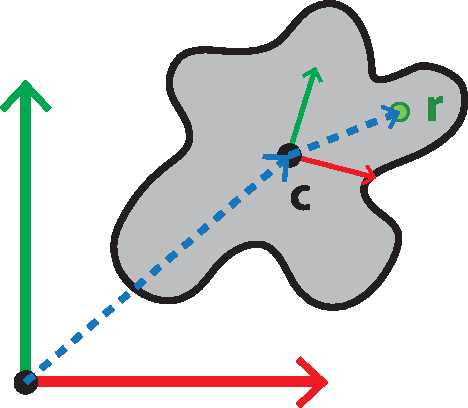
\includegraphics[width=.4\textwidth]{images/rigid_body_1.pdf}
\caption{Rigid body model illustration}
\label{img:rigid_body}
\end{figure}

By definition only the affine transformations of rotation and translation can apply to any rigid body. The main task of the rigid body simulation therefore is to calculate these two variables over time \(t\).

The physics behind the rigid body simulation is based on Newton's laws of motion. Most importantly the first law stating that if no force acts on an object, the velocity of the object will remain constant. Thus follows that the simulation has to model all forces acting on the body. These forces are the only causes for a change in the body's state and thus its position and orientation in space. The forces either cause a change in the linear velocity of the body, or an angular velocity results in a rotation of the body. 

The position of the rigid body is defined by the position $x(t)$ of its center of mass in world coordinates over time. The change of this position over time defines the linear velocity $v(t)$ for the body. So the linear velocity is simply the following:

\begin{equation}
v(t) = \dot{x}(t)
\end{equation}

The angular velocity is a more difficult to define. First the current rotation of the body has to be stated. The orientation of the rigid body was defined as unit quaternion $q(t)$. The change in orientation can then be calculated using the following:

\begin{equation}
\dot{q}(t) = \omega(t) * q(t)
\end{equation}

Here $\omega(t)$ denotes the angular velocity of the body at any point in time. Both the linear velocity and the angular velocity are integrated in every time step to simulate the body's behavior.

This mean, that the state of a rigid body in its most basic form is defined by just the following five variables:

\begin{align*}
m &, \text{the mass} \\
x &, \text{the position of the center of mass} \\
q &, \text{the orientation} \\
v &, \text{the linear velocity} \\
\omega &, \text{the angular velocity} \\
\end{align*}

Until now only the state of the rigid body has been defined. In the real world forces are acting upon the body, which cause a change in its state according to Newton's laws of motion. The most prominent forces usually modeled in a rigid body simulation are for example gravity, collision and friction. In the real world forces always act over a defined amount of time. Unfortunately for the simulation an instantaneous change in velocity is more desirable, so that for example in the case of collision the relative velocity of the involved bodies comes to a hold immediately. In order to achieve this goal, the new quantity $J$ is introduced. $J$ is called an impulse and represents a force integrated over time.

\begin{equation}
F \Delta t = J
\end{equation}

Letting $F$ go to infinity and $\Delta t$ to zero describes how the force would change the velocity as if it caused an immediate change. $J$ thus has the units of momentum. 

The effects of any impulse have to be evaluated for both the linear velocity as well as for the angular velocity. For the linear velocity the change is rather defined as

\begin{equation}
v(t) = \frac{P(t)}{M}
\end{equation}

In this case $P(t)$ denotes the linear momentum aggregated across all force acting upon the body and $M$ is simply the mass of the rigid body.

The formula for the angular velocity is slightly more involved

\begin{equation}
\omega(t) = L(t) * inv(I(t))
\end{equation}

Here $L(t)$ denotes the angular momentum. $I(t)$ is called the inertia tensor and is a simple scaling factor between the angular momentum $L(t)$ and $\omega(t)$ just like $inv(M)$ is in the linear case. The inertia tensor describes how the mass of the body is distributed relative to the body's center of mass. It depends on the orientation of the body but not on the translation.

Combining all the state variables with impulses yields the basic foundation for a rigid body simulation. A simplistic version of the simulation loop can for example look like this:

\clearpage

\begin{algorithm}[t!]
\caption{Rigid Body Simulation Loop}
\begin{algorithmic}[1]
\FORALL{bodies $b$}
	\STATE{apply gravity}
	\STATE{integrate velocities}
	\STATE{predict state}
\ENDFOR
\FORALL{bodies $b1$}
	\FORALL{bodies $b2$}
		\STATE{perform collision detection between body $b1$ and body $b2$}
	\ENDFOR
\ENDFOR
\FORALL{collisions $c$}
	\STATE{resolve collision $c$}
\ENDFOR
\FORALL{bodies $b$}
	\STATE{integrate position and orientation}
\ENDFOR
\end{algorithmic}
\end{algorithm}

\section{Shape Matching}
\label{sec:shape_matching}

Shape Matching is a geometrically motivated approach to simulating deformable objects and was invented by M{\"u}ller et al. in \cite{Muller:2005fi}. It describes objects as a collection of points and does not need connectivity information. By trading in physical correctness the technique is able to provide an unconditionally stable simulation. 

The main concept of this deformable model is to replace the system of forces and energies between the different particles by simple geometric constraints and distances. All points are moved to goal positions, which are obtained by shape matching the original rest state of the object to the currently deformed state of the object. These well-defined goal positions are computationally easy to obtain and provide an unconditionally stable simulation.

\begin{figure}[h]
\centering
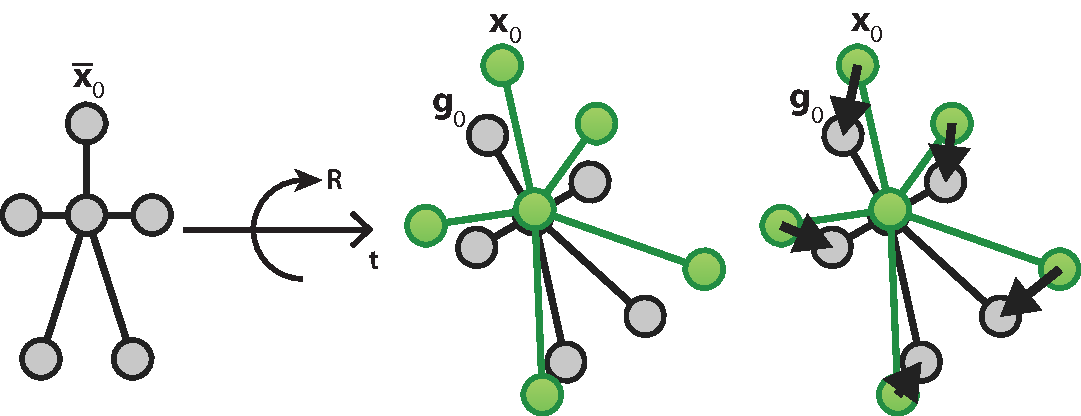
\includegraphics[width=.96\textwidth]{images/shape_matching.pdf}
\caption{Shape matching illustration}
\label{img:shape_matching}
\end{figure}

The algorithm only takes a set of particles and their initial configuration as inputs. Each particle has four variables:

\begin{align*}
m_i &, \text{the mass} \\
\bar{x}_i &, \text{the rest position} \\
x_i &, \text{the current position} \\
v_i &, \text{the velocity}
\end{align*}

The integration scheme uses the goal positions \(g_i\) to move the particles to the desired goal positions. The amount of movement can directly be modeled as a simple stiffness parameter \(\alpha\). A stiffness parameter of \(1\) thus basically does not allow for any deformation as the particles are always moved to their ideal transformed state. By using all this information and the external forces (i.e. gravity) the integration step becomes:

\begin{align}
v_i(t+h) &= v_i(t) + \alpha * \frac{g_i(t)-x_i(t)}{h} + h * f_{ext}(t)/m_i \\
x_i(t=h) &= x_i(t) + h * v_i(t+h)
\end{align}

The goal position \(g_i\) is obtained by shape matching the rest shape to the current deformed shape. The problem shape matching solves is thus defined by finding the rotation matrix \(R\) and the translation vector \(t\) between the two sets of points \(\bar{x}_i\) and \(x_i\). The desired matrix \(R\) and vector \(t\) minimize the following term:

\begin{equation}
\sum\limits_i m_i(R(\bar{x}_i-\bar{t})+t-x_i)^2
\label{eq:minimize_shape_matching}
\end{equation}

The optimal translation vectors are simply the respective center of masses of the rest shape and the deformed shape.

\begin{equation}
\bar{t} = \bar{c} = \frac{\sum_{i} m_i \bar{x}_i}{\sum_{i}m_i}, t = c = \frac{\sum_{i} m_i x_i}{\sum_{i}m_i}
\end{equation}

Unfortunately the optimal rotation matrix is not as simple to compute. The equation \ref{eq:minimize_shape_matching} has to be simplified. The first step is to define relative positions for all points with respect to their center of mass.

\begin{gather}
q_i = \bar{x}_i - \bar{c}, p_i = x_i - c \\
\sum\limits_i m_i(Rq_i-p_i)^2
\label{eq:center_of_mass_shape_matching}
\end{gather}

The next insight is to actually find the optimal linear transformation \(A\) instead of the optimal rotation matrix \(R\).  Calculating the derivative with respect to all coefficients of \(A\) and setting it to zero gives the optimal linear transformation.

\begin{equation}
A = (\sum_i m_i p_i q_i^\top)(\sum_i m_i q_i q_i^\top)^{-1}=A_{pq}A_{qq}
\end{equation}

\(A_{qq}\) is a symmetric matrix and therefore contains no rotational part. All the rotation is encapsulated in \(A_{pp}\). The optimal rotation matrix can now be found by calculating the polar decomposition \(A = RS\). This allows to finally write down the goal position for each particle as:

\begin{equation}
g_i = R(\bar{x}_i - \bar{c}) + c
\end{equation}

All particles are then moved to their respective goal positions by a variable fraction. This fraction effectively models the stiffness of the deformable body. If the stiffness fraction is close to $1$ the particles will practically snap to their ideal goal positions which by definition are not deformed as they only include translation and rotations of initial rest state. If the stiffness fraction however is very low the particles will stay in their predicted position and the body is completely deformed.

\section{Position Based Dynamics}
\label{sec:position_based_dynamics}

Position based dynamics (PBD) is a method which omits the traditional force based approach used in simulating dynamics systems but instead directly works on the positions to simulate deformable objects and was proposed by M{\"u}ller et al. in \cite{Muller:2007vs}. This means it also is not physically correct but instead provides an efficient unconditionally stable simulation. Like shape matching it also tries to satisfy constraints in order to arrive at stable end positions. However, instead of one global constraint, the shape, position based dynamics handles many different constraints. These constraints either model the physical properties of the object and are thus fixed throughout the simulation, or are generated on demand in the case of collision constraints used to resolve collisions. As the name also implies position based dynamics only works with the position of the particles updating them directly. The velocity of the particle is solely determined by the difference in positions overtime. This is best illustrated by the pseudocode of the simulation loop.

\begin{algorithm}[htb]
\caption{Position Based Dynamics Simulation Loop}
\begin{algorithmic}[1]
\FORALL{vertices $i$}
	\STATE{initalize $x_i=\bar{x}_i, v_i =\bar{v}_i, w_i = 1/m_i$}
\ENDFOR
\LOOP
	\FORALL{vertices $i$} \STATE{$v_i \gets v_i + \Delta t w_i f_{ext}(x_i)$}\ENDFOR
	\STATE{dampVelocities($v_1,...,v_N$)}
	\FORALL{vertices $i$} \STATE{$p_i \gets x_i + \Delta t v_i$}\ENDFOR
	\FORALL{vertices $i$} \STATE{generateCollisionConstraints$(x_i\rightarrow p_i)$} \ENDFOR
	\WHILE{$i \leq solverIterations$}
		\STATE{projectConstraints$(C_1,...,C_{M+M_{coll}},p_1,...,p_N)$}
	\ENDWHILE
	\FORALL{vertices $i$} 
		\STATE{$v_i \gets (p_i-x_i)/\Delta t$}
		\STATE{$x_i \gets p_i$}
	\ENDFOR
	\STATE{velocityUpdate$(v_1,...,v_N)$}
\ENDLOOP
\end{algorithmic}
\end{algorithm}

The first key insight into the algorithm occurs in lines 9-11. Here positions for all vertices are estimated using the current velocity and the time step. This step is completely unrestricted and just predicts and estimates a position which is then later redefined. Line 15-17 illustrate this refinement. A Gauss-Seidel type iteration is used to satisfy all constraints defined for the system. These constraints mostly model the inherent structure of the object currently simulated but another important aspect handled here are collisions, which are just another constraint for the system and generated in each time step after estimating the position. The idea is to iterate over all constraints multiple times so that the particles are projected to valid locations with respect to the given constraint. The final vital piece of the algorithm can be seen in lines 18-21. After all constraints have been satisfied as good as possible the estimated positions alone are used to update the state of all vertices. The velocity of the particle is solely calculated by the difference of the new estimated position and the former position. This integration scheme is unconditionally stable as it does not just extrapolate into the future like traditional explicit schemes do. Instead it uses the physically valid positions computed with the constraint solver.

\clearpage
\section{Oriented Particles}
\label{sec:oriented_particles}

\begin{figure}[htb]
\centering
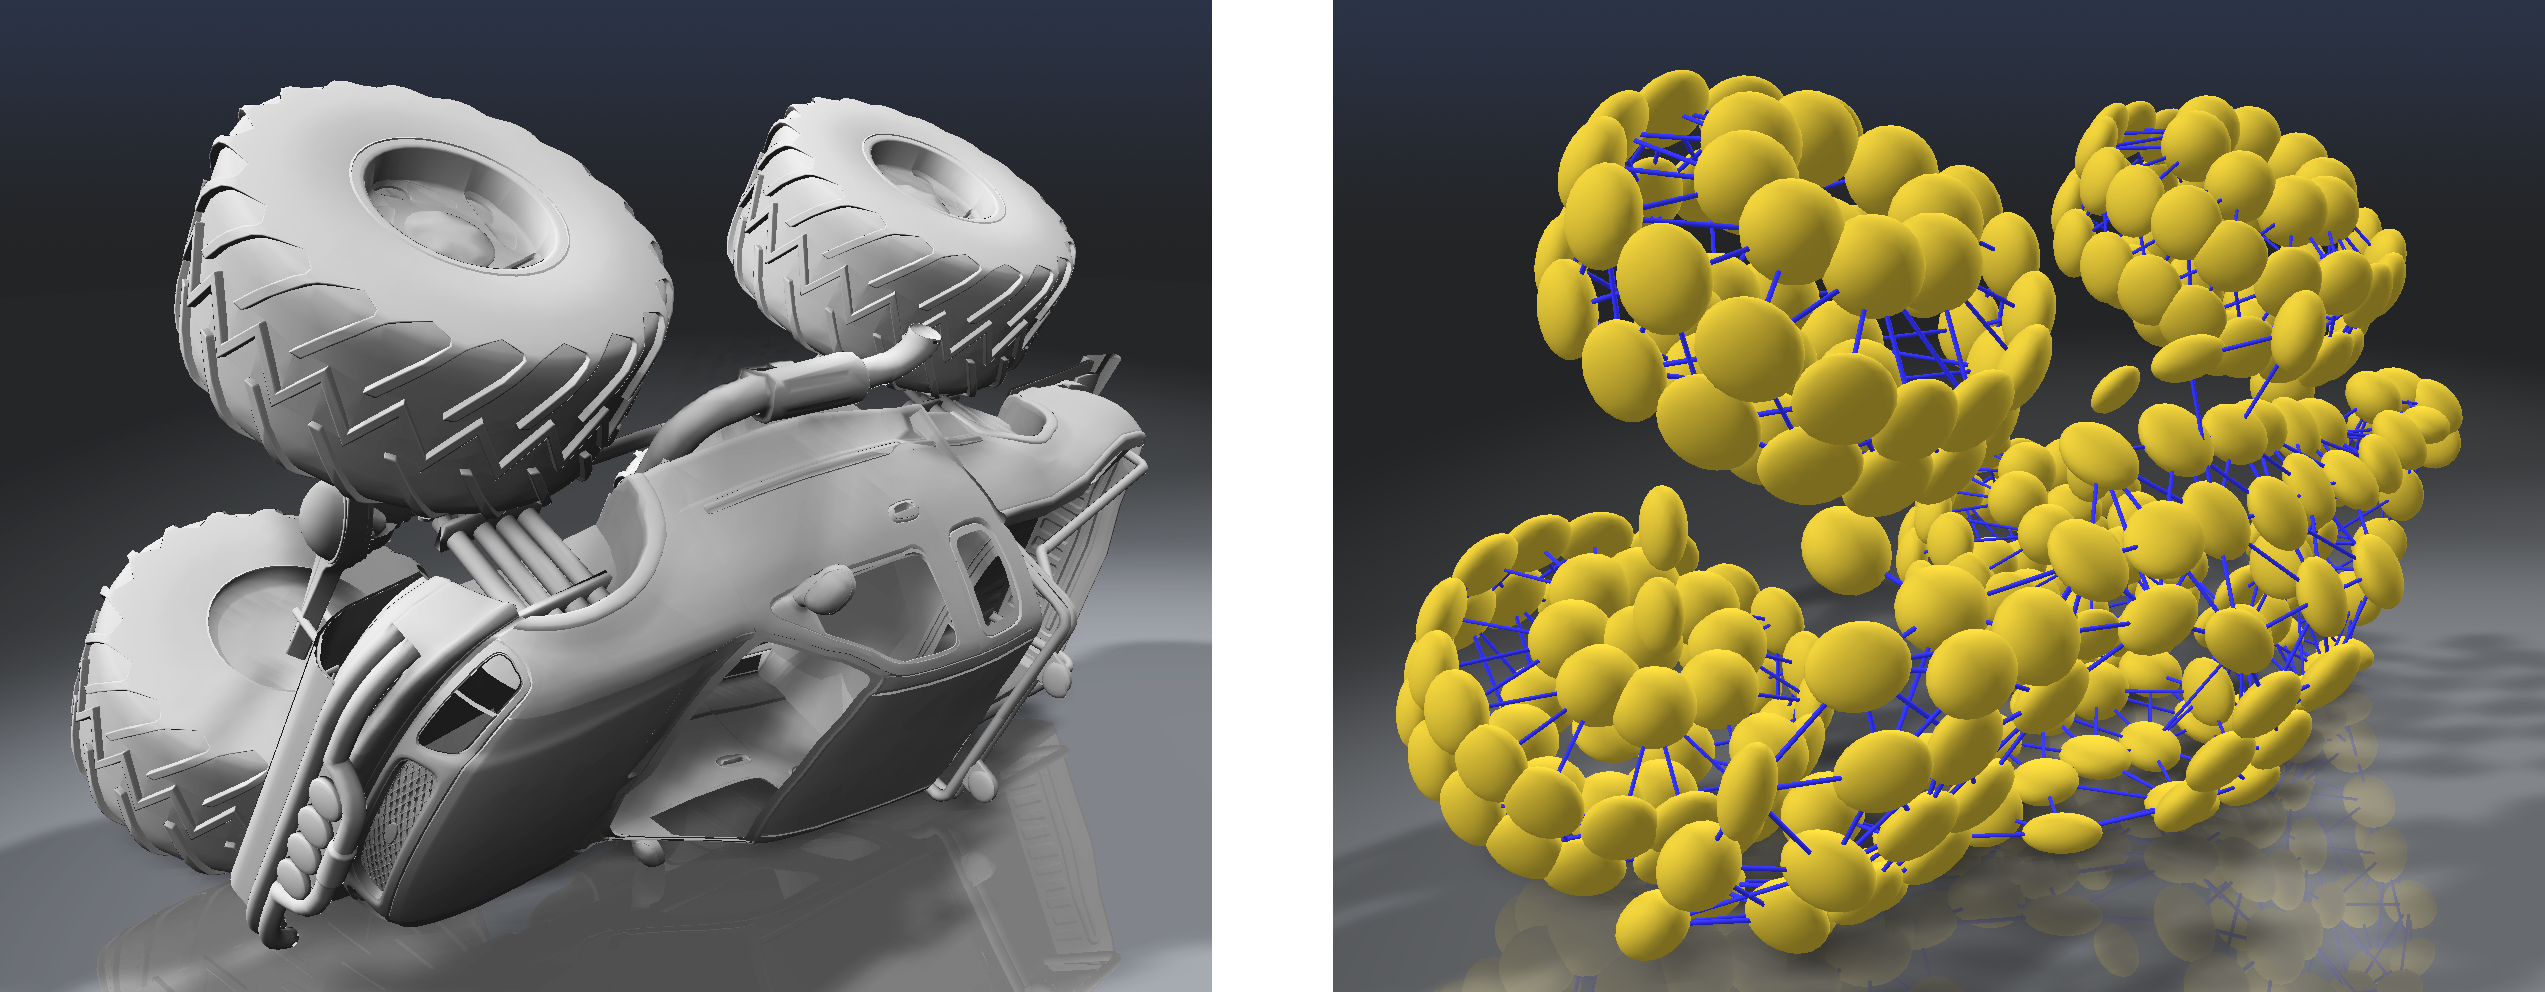
\includegraphics[width=.8\textwidth]{images/oriented_particles_illustration.png}
\caption[Oriented particle illustration]{Oriented particle illustration\cite{Muller:2011gn}}
\label{img:oriented_particles_illustration}
\end{figure}

Oriented particles as described by M{\"u}ller et al. \cite{Muller:2011gn} combine the geometrical based approach of shape matching with the idea of updating the velocities based on the positions alone as described in position based dynamics. They specifically improve upon shape matching in sparse regions increasing the overall stability of the shape matching. Modeling the particles as oriented ellipsoids can approximate the surface more accurately than simple sphere, which is especially useful in calculating and resolving collisions.

\subsection{Generalized Shape Matching}
The main idea is to use oriented particles which also store rotation and spin, in addition to the position and velocity. The particles now all have orientation information associated with them, thus the name of the method. The variables for each particle are thus extended to encompass the following seven variables:

\begin{align*}
m_i &, \text{the mass} \\
\bar{x}_i &, \text{the rest position} \\
\bar{q}_i &, \text{the rest orientation} \\
x_i &, \text{the current position} \\
q_i &, \text{the current orientation} \\
v_i &, \text{the linear velocity} \\
\omega_i &, \text{the angular velocity}
\end{align*}

The advantages of including orientations for each particle become particularly evident in sparse regions of the model like for example chains of particles or even single particles. The traditional approach of using spherical particles to model twisting chains would involve adding many particles to capture the twist. In order to model the same scenario with oriented particles only a single particle is required as the twisting is completely captured in the rotation and spin of the particle.

\begin{figure}[htb]
\centering
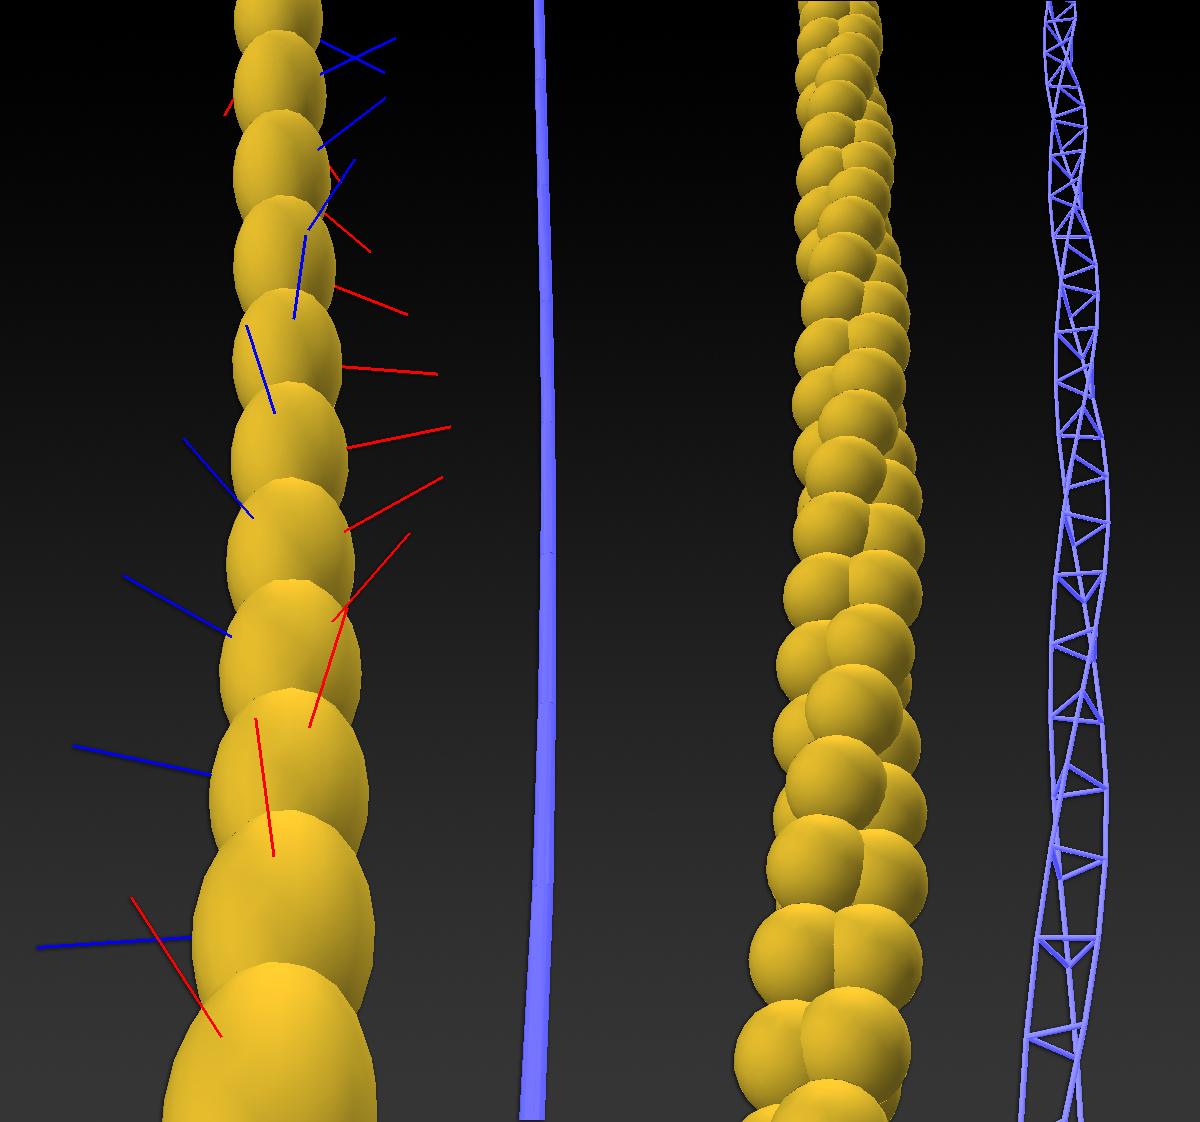
\includegraphics[width=.5\textwidth]{images/oriented_particle_twist_chain.png}
\caption[Oriented particle twisting chain]{Oriented particle twisting chain\cite{Muller:2011gn}}
\label{img:oriented_particle_twist_chain}
\end{figure}

The basic approach of shape matching is directly applied to the generalized shape matching used for the oriented particle but differs in the way the moment matrix is calculated. The original minimization function \ref{eq:minimize_shape_matching} is slightly modified so it becomes the following moment matrix $A$, but is essentially still the same as in the original shape matching approach.

\begin{equation}
A = \sum\limits_i^n m_i(x_i-c)(\bar{x}_i - \bar{c})^\top  \in \mathbb{R}^{3x3}
\label{eq:minimize_oriented_particle_1}
\end{equation}

This moment matrix $A$ in terms of $n$ particles each with a corresponding mass $m_i$ and current position $x_i$. The center of mass for the current configuration is defined as $c$. Analog to that the rest position is defined as $\bar{x}_i$ and the rest center of mass as $\bar{c}$. Both center of mass are calculated using the traditional approach as seen in equation \ref{eq:center_of_mass_shape_matching}.

Just like in the original shape matching approach the goal is to find the optimal translation vector $t$ and rotation matrix $R$, which map the original shape to the current configuration in a least squares manner. The optimal translation vector can simply be calculated from the differences of the two centers of mass.

\begin{equation}
t = c - \bar{c}
\end{equation}

The rotation matrix $R$ can be obtained by calculating the polar decomposition of $A$

\begin{equation}
A = R*S
\end{equation}

Together with translation vector $t$ and the extracted rotation matrix $R$ the goal positions for each particle can be calculated.

\begin{equation}
g_i = R(\bar{x}_i-\bar{c})+c
\end{equation}

Thus far this is still exactly the same as in the original shape matching approach. Unfortunately  the moment matrix $A$ can become ill-conditioned or even singular. This happens if the particles are close to co-planar or as in the example of the twisting chain co-linear. If $A$ is ill-conditioned the polar decomposition is not well defined and yields only unusable and unstable results. Thus no reliable $R$ can be obtained. Adding the orientation information for each particle into the calculation can fix this problem.

The solution involves defining a well-conditioned moment matrix for even single particle and consequently adding each moment matrix together in order to arrive at a total moment matrix for the whole particle group. In order to get to this result let's begin with two groups of particles, each with their own unknown moment matrix $A_1$ and $A_2$ respectively. Both moment matrices are defined with respect to their own center of mass and thus cannot simply be added to arrive at the combined moment matrix. As described in Rivers et al. \cite{Rivers:2007te} equation \ref{eq:minimize_oriented_particle_1} can be reformulated to the following formula which shifts the center of mass to the global one.

\begin{equation}
A = \sum\limits_i^n m_ix_i\bar{x}_i^\top - Mc\bar{c}^\top
\label{eq:minimize_oriented_particle_2}
\end{equation}

Here $M$ is simply defined as the sum of all particle masses. Now the next step is to apply the same logic to each individual particle forming the group instead of two separate groups. This yields the following equation

\begin{equation}
A = \sum\limits_i^n (A_i + m_ix_i\bar{x}_i^\top-m_ic\bar{c}^\top)
\end{equation}

$A_i$ denotes the moment matrix for a single particle in the group while the other variables retain their original meaning. This equation can be generalized and improved further.

\begin{equation}
A = \sum\limits_i^n (A_i + m_ix_i\bar{x}_i^\top) - Mc\bar{c}^\top
\end{equation}

Integrating the equation \ref{eq:minimize_oriented_particle_1} over the particle's volume yields the moment matrix for a single particle. Each particle is modeled as an ellipsoid so their moment matrix is defined in terms of their radii and rotation.

\begin{equation}
A_{\text{ellipsoid}} = \frac{1}{5}m \begin{bmatrix} a^2 & 0 & 0 \\ 0 & b^2 & 0 \\ 0 & 0 & c^2  \end{bmatrix} R
\end{equation}

The radii of a single particle are simply defined by the length of the semi-axes $r = [a,b,c]^\top$ in all orthonormal directions. Including the orientation $R$ for each single particle causes the total moment matrix $A$ to always be full ranked and thus the polar decomposition to return more reliable results.

Having defined a stable moment matrix for each group the optimal translation vector and rotation matrix can be obtained and thus the goal positions can be calculated. Again analog to the original shape matching the particles are pulled towards their goal positions by a variable stiffness fraction. However the oriented particles' way of integrating the position and velocities of the particles is completely different from the way the traditional shape matching method works. Instead the oriented particles are updated and integrated by a system closely modeled after the position based dynamics' approach but extended by integrating the orientations of the particles.

\subsection{Generalized Position Based Dynamics}
As in Position Based Dynamics (PBD) the first step is the prediction step. Here a new predicted position $x_p$ is calculated for each particle using a simple integration scheme. However for oriented particles the associated orientation $q_p$ of each particle also has to be predicted over time. This prediction step using an explicit Euler integration looks like the following:

\begin{align}
x_p &\leftarrow x + v\Delta t \\
q_p &\leftarrow [\frac{\omega}{|\omega|}sin(\frac{|\omega|\Delta t}{2}), cos(\frac{|\omega|\Delta t}{2})]q
\end{align}

Now the solver has calculated a predicated state $(x_p,q_p)$ for each single particle. This information is then based onto the second step. The second step is simply the adaptation and modification of the predicted state according to the rules laid out by the generalized shape matching approach outlined above. The last and final step is to integrate the state for each particle. In accordance with PBD but in difference to shape matching the integration step only takes in the particle's state in the beginning of the iteration and the adjusted predicted state. This way, like in PBD, calculating the velocities is solely based on the positions and orientations provides an unconditionally stable scheme as the adjusted predictions never overshoot. The integration step thus becomes the following equations:

\begin{align}
v &\leftarrow (x_p - x)/\Delta t \\
x &\leftarrow x_p \\
\omega &\leftarrow axis(q_p q^{-1}) \cdot angle(q_p q^-1)/\Delta t \\
q &\leftarrow q_p
\end{align}

The function $axis(q)$ simply returns the normalized direction of the quaternion $q$ and $angle(q)$ consequently the angle. One caveat to take note of is the observation that there are always two possible rotations $r=q_pq^{-1}$ to transform $q$ into $q_p$. It is important to choose the smaller rotation of the two to update the angular velocity $\omega$.

The standard simulation model for oriented particles uses an implicit shape matching. For implicit shape matching the particle belonging to an implicit shape matching group are defined by their edges. A group exists for every particle at the center and additionally all the particles connected to this center particle by an edge. The results of this usually look like a tetrahedral mesh in more connected regions and thin particle chains in very sparse regions. However the topology of the particles can be completely arbitrary.

In practice a Gauss-Seidel type iteration scheme is used to satisfy all shape matching constraints defined by the implicit groups. This reduces the effect of the inherent bias towards the first groups that are evaluated during the execution. After updating the predicted state multiple times taking into account all groups the predicted position of each particle is moved towards the calculated goal position by a stiffness fraction. The orientation however is only updated for the respective center particle.

\subsection{Collision Handling}
\label{subsec:collision_handling}

Another improvement oriented particles provide is a more accurate collision handling. Each oriented particle is no longer a simple sphere but instead is modeled as an ellipsoid.

\begin{figure}[htb]
	\centering
	\subfigure[Sphere collision]{
		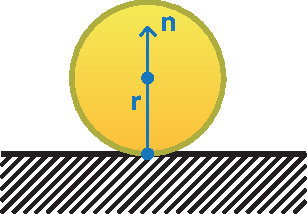
\includegraphics[width=.3\textwidth]{oriented_particles_collision_sphere.pdf}
		\label{subfig:collision_sphere}
	}
	\subfigure[Incorrect ellipsoid collision]{
		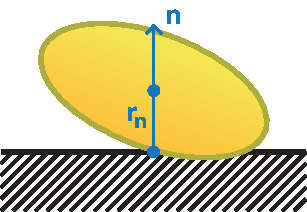
\includegraphics[width=.3\textwidth]{oriented_particles_collision_ellipsoid_wrong.pdf}
		\label{subfig:collision_ellipsoid_incorrect}
	}
	\subfigure[Correct ellipsoid collision]{
		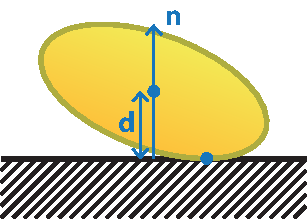
\includegraphics[width=.3\textwidth]{oriented_particles_collision_ellipsoid_correct.pdf}
		\label{subfig:collision_ellipsoid_correct}
	}
	\caption{Particle collision handling}
	\label{fig:collision_handling}
\end{figure}

Ellipsoids can fit to the surface area of a model better than simplistic spheres can. Using spheres might cause unnatural frictions or other visual artifacts. The question now remains how to calculate the correct spot on the surface of the ellipsoid that collided with a plane as can be seen in figure \ref{subfig:collision_ellipsoid_correct}. The simplistic approach used in the spherical case cannot directly be transferred as illustrated in figure \ref{subfig:collision_sphere} and \ref{subfig:collision_ellipsoid_incorrect}. This would only work if the contact normal was aligned to the principal axis of the ellipsoid. However, in almost all cases this is not true and the calculation becomes a little bit more involved.

Each potential particle is defined by its principal radii $a,b,c$ and its rotation matrix $R$. The potential collision plane is simply defined in hessian form as $p = n^\top x=d$. The first step is to compute the contact point on the surface of the ellipsoid with a normal that is parallel to the normal of the plane $n$. In general the ellipsoid can be defined in terms of the following zero iso-surface:

\begin{equation}
c(x) = x^\top A x - 1
\end{equation}

The potential contact point has to meet the following two constraints:

\begin{align}
\nabla c(x)&=\lambda n \\
c(x) &= 0
\end{align}

In addition to these two constraints the following two formulas yield enough information to solve for $\lambda$ and $x$, though only $x$ is of real interest.

\begin{align}
\nabla c(x)&=2 A x \\
A = R \begin{bmatrix}\frac{1}{a^2} & 0 & 0 \\ 0 & \frac{1}{b^2} & 0 \\ 0 & 0 & \frac{1}{c^2}\end{bmatrix} R^\top &\Rightarrow A^{-1} = R \begin{bmatrix}a^2 & 0 & 0 \\ 0 & b^2 & 0 \\ 0 & 0 & c^2\end{bmatrix}R^\top
\end{align}

Thus $\lambda$ and $x$ can be calculated in the following manner:

\begin{align}
\lambda &= \pm \frac{2}{\sqrt{n^\top A^{-1} n}} \\
x &= \pm \frac{A^{-1}n}{\sqrt{n^\top A^{-1} n}}
\end{align}

These calculations always lead to two possible positions $x$ on the surface of the ellipsoid, which have a normal parallel to the plane normal. The correct point to choose is always the point which is closer the plane. This can easily be calculated given the hessian form of the plane. The final step to determine if a collision between the current particle and the plane has occurred is to check if the contact point is below the plane and thus satisfies the condition $n^\top x < d$. Solving this condition also automatically returns the penetration depth of the collision. The depth can directly be utilized to modify the predicted position of particle. The collision detection and resolution step is done for all particles after the positions have been predicted but before the shape matching. Although the collision step should ideally be calculated for every iteration, using Gauss-Seidel, of the shape matching, this is way too expensive as the number of particles and planes can get quite large very quickly. However, just resolving the collisions once before shape matching seems to give satisfactory results.

The oriented particles paper describes a couple of additional features for the simulation with oriented particles. These include explicit shape matching groups defined manually, plastic deformation which cause the rest state to change, friction, torsion resistance, stretching and bending, collision handling between two ellipsoids and using the orientation information for more efficient skinning. However, these features are not needed to achieve the goals and requirements of this thesis and are thus not described here. More details can be found in the original paper.